\documentclass[varwidth=40cm]{standalone}
\usepackage{tikz}
\usepackage{style}

\let\r\undefined
\newcommand{\r}[2]{\draw[fill=lightgray] (#1,0) rectangle (#1+1,#2);}

\begin{document}
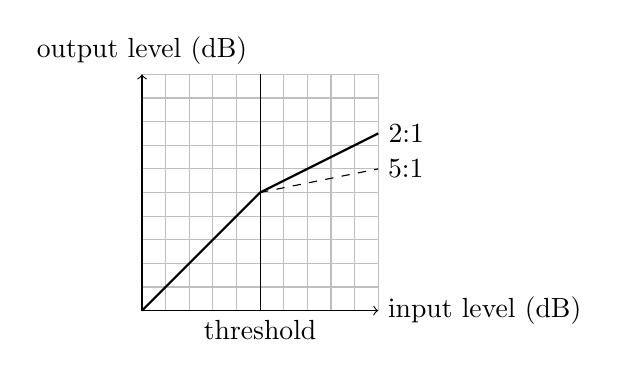
\begin{tikzpicture}[scale=0.3]
  \foreach \i in {0,...,10} {
    \draw[lightgray] (0,\i) -- (10,\i);
    \draw[lightgray] (\i,0) -- (\i,10);
  }
  \draw (5,0) node[below] {threshold} -- (5,10);
  \draw[->] (0,0) -- (10,0) node[right] {input level (dB)};
  \draw[->] (0,0) -- (0,10) node[above] {output level (dB)};
  % \draw[dotted] (5,5) -- (10,10) node[right] {1:1};
  \draw[thick] (0,0) -- (5,5) -- (10,7.5) node[right] {2:1};
  \draw[dashed] (5,5) -- (10,6) node[right] {5:1};
\end{tikzpicture}
\end{document}
